\begin{doublespace}
After completing all components of the project, including all programming and user studies, we can evaluate the project to determine whether our goals were met. Since a major part of this project was to make the program easy to use (by following HCI, human computer interaction, metrics and heuristics as described in Chapter~\ref{sec:lit}), an evaluation of these metrics is also needed. Finally, there are some parts of the program which are incomplete or need extra work. Those incomplete parts, as well as any extra features that could be added in the future, will be described in this section.

\subsection{Project Evaluation}
After a large project such as this one, it is important to evaluate the outcome of the project to see if all the goals that were set at the beginning were met. A description of our goals and requirements can be found in Chapter~\ref{sec:req}. In summary, our goals were:
\begin{itemize}
    \item Convert the existing gear train design software from Windows Forms to WPF
    \item Create a 3D previewer of the user's gear train design
    \item Run user studies using the old system and GearTrain to gather user feedback
\end{itemize}

After project completion, we \textbf{successfully converted} the old gear design software from Windows Forms to WPF. This required a complete rewrite and redesign of the UI (Chapter~\ref{sec:design_ui}), but the benefits of this new graphics framework outweighs the cost of rewriting the UI. WPF is newer, has better performance (especially for graphics-intensive programs such as the 3D viewer), has many more options for possible UI controls, and continues to receive updates from Microsoft.  

The 3D previewer of the gear design is \textbf{partially implemented}. The 3D viewer shows the general structure of the gears, however it is not completely accurate. The main issue is that the shapes are not actual gears. They are simple shapes like cylinders and disks. A future project team could implement the 3D viewer to contain real gear and bearing shapes. The second issue is that the shaft and bearing locations do not always match the SolidWorks generation. This is due to an issue with how shafts are represented in the code. This problem existed in the old system as well. A future team could fix this shaft issue and thus fix the 3D viewer as well as some SolidWorks generation issues relating to shafts.

After project completion, we had run a total of \textbf{three user studies} to evaluate and compare the old system with GearTrain. As explained in Chapter~\ref{sec:eval}, users generally found GearTrain to be easier to use than the old system, and most users found that the 3D viewer improved their experience. Participants in these studies gave us feedback about which features should be added in the future. Some of these will be explained in Section~\ref{sec:futurework}. All feature requests can be found in Appendix~\ref{app:survey}.

\subsubsection{Heuristic Evaluation}
In Chapter~\ref{sec:lit}, we talked about HCI metrics and heuristics which can be used to evaluate a system. The ten heuristics are first described in Table~\ref{tab:heuristics}, while Table~\ref{tab:heur_eval} explains how every heuristic was met by GearTrain.

\begin{singlespace}
\begin{table}[htbp]
    \caption{UI heuristic evaluation.}
    \label{tab:heur_eval}
    \begin{tabularx}{1\textwidth}{||Y|Y||}
         \hline \textbf{Heuristic} & \textbf{Evaluation}  \\ \hline \hline
         Visibility of system status & Users can always see the state of their design using the 3D viewer, no matter where they are in the application. \\ \hline
         Match between system and the real world & Proper gear terminology is used (e.g., ``Bevel'', ``Pitch''). \\ \hline
         User control and freedom & User is always able to navigate between screens using back or cancel buttons. Shaft and gear editing allows the user to undo their work if they make a mistake. \\ \hline
         Consistency and standards & UI element design (color, shape) are consistent throughout the application. Terms are only repeated when referring to the exact same object. \\ \hline
         Error prevention & System checks for bad input from the user and warns them about errors or mistakes. System does not allow users to create an invalid gear train design. \\ \hline
         Recognition rather than recall & Most actions in the application are available all the time (and are dynamically enabled/disabled depending on system state), so the user always knows when they are allowed to do something. \\ \hline
         Flexibility and efficiency of use & The system has features for both advanced and novice users, such as SolidWorks-like 3D viewer controls (advanced) and tooltips (novice). \\ \hline
         Aesthetic and minimalist design & The interface was designed to only have the elements that it absolutely requires with nothing extra. \\ \hline
         Help users recognize, diagnose, and recover from errors & Anytime an error happens, such as if the users has incorrect input or a problem opening a file, an error popup appears. This error popup tells the user (1) what the error is, (2) what caused it, and (3) how to fix it. \\ \hline
         Help and documentation & Every UI element has a tooltip explaining what it is and how to use it. A help website was also created in case the user needs extra help. \\ \hline
    \end{tabularx}
\end{table}
\end{singlespace}

\subsection{Project Experience}
The MQP is the culmination of a student's learning at WPI (the ``capstone''). As such, it requires us to apply knowledge from almost every class that we have taken. Each of us having taken different courses with different prior experience, we were able to figure out our own individual skills and how they are applied to the project.

\subsubsection{Applied Skills}
The main skill that was used was both of our knowledge using the \textbf{C\# programming language}. Although there is not a single course at WPI that teaches or uses this language, we both had much experience using it in our own personal programming projects. We both had used \textbf{WPF} extensively in the past, so creating a UI in WPF and a backend in C\# was a good example of this skill. C\# is very similar syntactically to Java, a language used extensively at WPI classes and in the real world, so it is very easy to learn if one is already familiar with Java or another C-based language.

The final MQP report was written in \textbf{Latex} since it is very easy to format the document. Even more helpful was Latex' way of keeping track of figures and section numbers throughout the paper that would be very difficult to maintain if writing using a different format. Kyle has used Latex extensively in the past for homework assignments or other writing, so he was able to create the skeleton for the paper which both team members can fill in with writing.

A large part of the project was based on UI improvements, as well as user experience improvements. Since many users of the old system found it hard to use, it was important to create a system which considered HCI principles. Alan had taken the HCI course at WPI previously, so he took charge of the \textbf{user interface design}, and thus knew what aspects of it were acceptable or needing improvement.

One of our main requirements, as well as how we evaluated our system, was to run a \textbf{user study} of the systems. Each study was almost identical to each other, and a study methodology needed to be created so that we knew what needed to be done to get the best results. Kyle's IQP (interactive qualifying project, a Junior-year project) was entirely focused on running a user study to compare groups of participants. That knowledge was used in creating the studies for this project. Some data analysis methods from his IQP were also used, such as different statistical functions.

Finally, we desired to create a help website for the software so that users have an easy way to get help with the software. In the previous system, there was no help whatsoever, making the software even harder to use. Alan used his knowledge of \textbf{web development} to create a help website for GearTrain, which many users consulted during the D21 study.

\subsubsection{Acquired Skills}
Besides applying all of our skills and knowledge from our college experience, the MQP is also a teaching experience. The skills we already have are applied, but new skills are acquired. This section will discuss some of those skills.

Being Computer Science students, we had never officially learned about \textbf{gears} before this project. We had a very basic understanding of what gears were and what they did, but did not have any knowledge of any gear terminology or other advanced aspects of gears. As seen in Chapter~\ref{sec:lit}, much research about gears was required in order to implement a system used for designing gears.

Even though we had some knowledge of \textbf{user interface design}, we learned much more about it during this project. Designing the UI required many aspects to be considered, including ease of use (for many different types of users), learnability, aesthetics (which colors are used, style of different UI elements), and more (see Chapter~\ref{sec:design_ui}). While working on our own projects or projects for classes, we never really needed to consider these HCI principles since that was not the focus. However, it was the focus of this project so it was very important that we had a solid understanding.

Finally, the main thing we learned was \textbf{project planning}. For each term, we needed to create a plan for the term. This plan helped us keep track of what tasks needed to be done, but also helped us determine whether we were on track to meet our goals or not. We created a Gantt chart for B and C term to help us plan our programming, user study, and writing goals. A Gantt chart is a type of bar chart which shows tasks on a timeline, with the person who is responsible for the task as well as task dependencies (\cite{clark_gantt_1922}). This significantly helped us achieve our goals since we had written down exactly what needed to be done by what date.

\subsection{Future Work}
\label{sec:futurework}
Throughout the project, we worked to convert the previous gear train design software from Windows Forms to WPF. While that and other major goals were completed, there were a few things we were unable to fully complete due to time constraints. There are some issues that exist with GearTrain that need to be fixed in the future. Additionally, participants from our user study recommended additional features which can be added.

\subsubsection{Unfinished Features}
This section will describe those features that we began to implement but were unable to finish, due to time constraints or other factors. These include bugs or just features that we started and were not able to finish.

\noindent\textbf{3D Gear Preview}

\noindent As discussed at the beginning of this chapter, the current 3D viewer can only draw simple shapes, such as cylinders, to represent gears. An accurate drawing of gears, including teeth and a proper bore, could be implemented with the 3D viewer to make the preview even more similar to what SolidWorks will generate.

Additionally, the ``Export to STL'' feature exports the entire model as one large STL file instead of as individual parts. When 3D printing an object, you generally print each part separately (so that the gears can move). Since this STL has all parts attached, it is unable to be 3D printed since the parts would not be able to move.

\noindent\textbf{Gear Analysis}

\noindent A gear and shaft analysis was proposed at the beginning of the project. There existed gear analysis code from a previous project worked on by Professor Radhakrishnan that could be used for this purpose. Simple input and output windows were created for gear analysis (described in Chapter~\ref{sec:design_ui}). This gear analysis code just needs to be integrated to use the UI windows for input and output. Additionally, a feature would need to be added to save the analysis results to a CSV file which an engineer could use for their own purposes.

\noindent\textbf{Shaft Backend Problems}

\noindent The way that shafts are represented in the backend code does not work well when multiple gear sets are added. This has been a problem since the previous software. When more gear sets are added, the default values for gear and bearing locations are set to values that are not actually on the shaft. Additionally, an issue with the SolidWorks generation code causes the shafts to generate incorrectly.

Figure~\ref{fig:broken_shaft} shows two issues with shaft generation. The first is that one shaft was placed far away from the rest of the shafts, already making the gear train invalid (and much different from what the user entered). The second issue is the size of the shafts. All the shafts in this image are extremely small, although it looks like all the gears and bearings are just really big. Because of this issue, all the gears were placed inside of each other, even though the ``Auto Mesh'' feature was used. This shaft problem is a major bug which makes it so users cannot edit shafts without risk of a problem.

\begin{figure}[htbp]
    \centering
    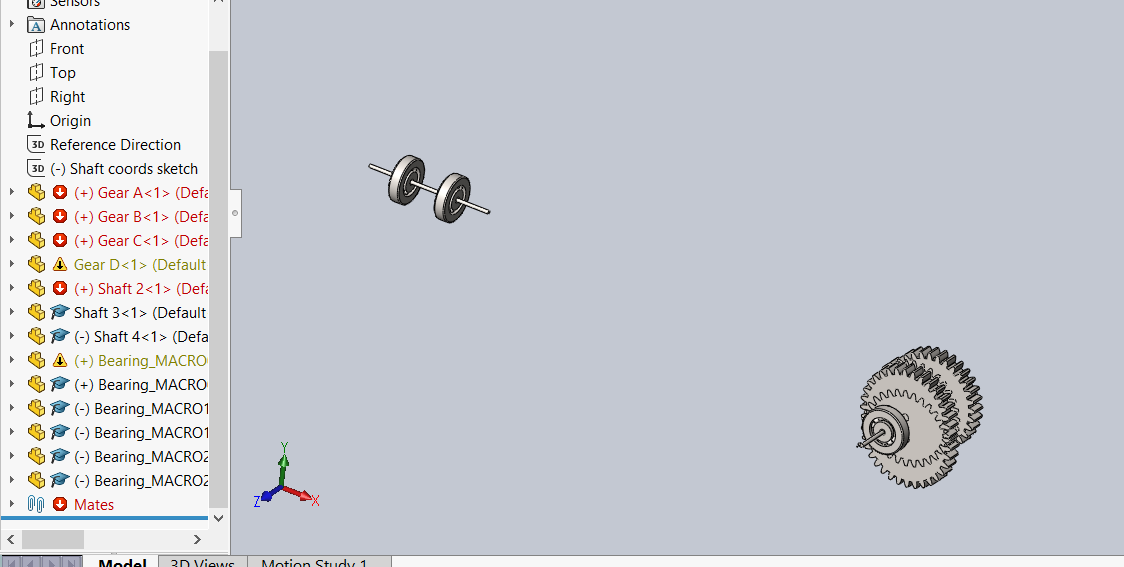
\includegraphics[width=\textwidth]{broken_shaft}
    \caption{Shaft generation error.}
    \label{fig:broken_shaft}
\end{figure}

\noindent\textbf{SolidWorks Generation Crashes}

\noindent As discusses in Chapters~\ref{sec:data} and \ref{sec:eval}, our user study required that users fully close out of SolidWorks before starting the generation. This is due to an issue in the \texttt{SolidWorksMacro.cs} file which can cause the program to crash in the middle of generation. The only way to fix it seems to be by fully closing SolidWorks before generating. A potential fix was implemented by making sure that \texttt{SolidWorksMacro} fully closes every file after it is done with it, but this did not fix it. This was the main issue with GearTrain that was reported by our users.

\subsubsection{New Features}
Finally, we will discuss new features that could be implemented in the future. Some of these features were recommended by participants in our user study, while others were from the project discussions about the software. Only those features from our discussions will be presented here. See Appendix~\ref{app:survey} for the features recommended by our users.

\noindent\textbf{GearTrain Installer}

\noindent Creating GearTrain as an installer instead of a standalone executable has been discussed. An installer would allow for the program to always be on the computer, which is easier for the user than having to keep GearTrain in a well-known location. This also allows for easy uninstallation by the Windows uninstall service. 

Another feature that was desired (and requested by a small number of users) was to allow users to double-click on a GearTrain design file and have it automatically open in GearTrain. This is possible, and is very common with other programs. However, this requires installation to the system because the operating system (Windows) needs to create a filetype association internally. Currently, users must open GearTrain, select File$\rightarrow$Open, and select a GearTrain design file to open. An easier way is to have the user double-click a GearTrain design file in their file explorer and the program opens automatically.

Installation is not possible at the moment because WPI IT services are strict on what programs can be installed to school computers. Before a program can be installed, it must be approved, which can take a long time or it may not be accepted at all.

\noindent\textbf{Automatically Find SolidWorks Location}

\noindent While GearTrain is able to look in the default SolidWorks install directory, it will not be able to find the program if the user chose to install it somewhere else. Although GearTrain saves the SolidWorks location that is provided by the user, if the user forgot where they installed it initially they may not be able to provide the location to GearTrain. Without the location of SolidWorks, the generation cannot be run. Similar to how Windows is able to find programs using the ``Search'' feature, a new feature could be to use that same functionality to find the SolidWorks executable. This would make it much easier for the user in case they do not know where SolidWorks is installed.

\end{doublespace}